\documentclass[12pt, letterpaper]{article}
\usepackage{graphicx}
\usepackage[T1]{fontenc}
\usepackage[polish]{babel}
\usepackage[utf8]{inputenc}

\graphicspath{{images/}}

%--------------------------------------------------------------------------------------------------
%       TITLE SECTION
%--------------------------------------------------------------------------------------------------
\begin{titlepage}
 

\includegraphics[scale=0.2]{ur_inf_logo}\\ \\ \\ \\

\begin{center}
	{ \huge \bfseries Technologie internetowe}\\[0.4cm] 

	\textsc{\Large Szablon strony HTML + JavaScript}\\[0.5cm] \\ \\ \\ \\ 
	
	\vspace{0.8cm}	
	
	\emph{Autor:} \\
	\textbf{Oskar Paśko} (117987)\\
	
	
	\vspace{0.8cm}
	
	\emph{Kierunek:} \\
	Informatyka i ekonometria
	
	\vspace{8cm}
	
	\emph{Prowadzący:} \\
	dr Katarzyna Gawrol\\ \\ \\ \\ 
	
	\vspace{2cm}
	
	Rzeszów, 2023
\end{center}
\end{titlepage}

\begin{document}

\section{Opis projektu}

\quad Projekt dotyczy walidacji danych podczas rejestracji użytownika. Walidacja zakłada, że wszystkie pola zostaną wypełniona. Walidacja sprawdza czy w polu imienia i nazwiska nie zostały wprowadzone cyfry. W polu email sprawdzany jest stan czy istnieje znak '@' w wpisanych adresie. Ponadto na końcu walidacja sprawdza czy podane hasła są takie same. W przypadku źle wpisanych danych lub przy braku wpisanych danych pojawiają się odpowiednie informację na temat źle wpisanych danych.\\ Po poprawnie wpisanych danych użytkownik zostanie przekierowany do podstrony 'hello.html' gdzie zobaczy informację o poprawnej rejestracji użytkownika.

\section{Struktura aplikacji}

\subsection{Strona Główna}

\begin{center}
	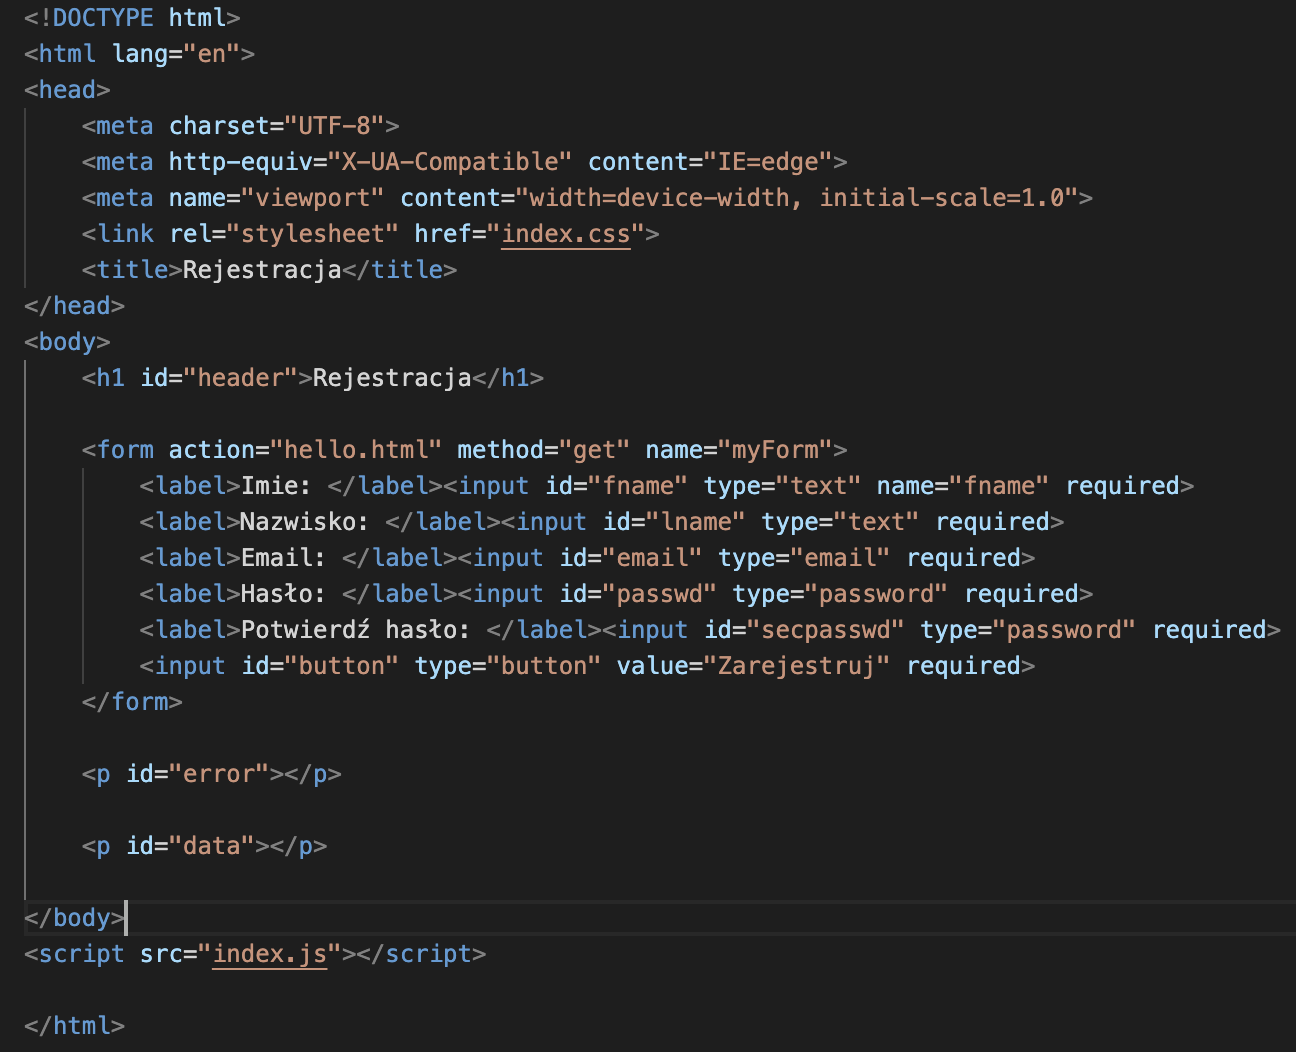
\includegraphics[scale=0.5]{index}
\end{center}

\subsection{Podstrona z powitaniem}

\begin{center}
	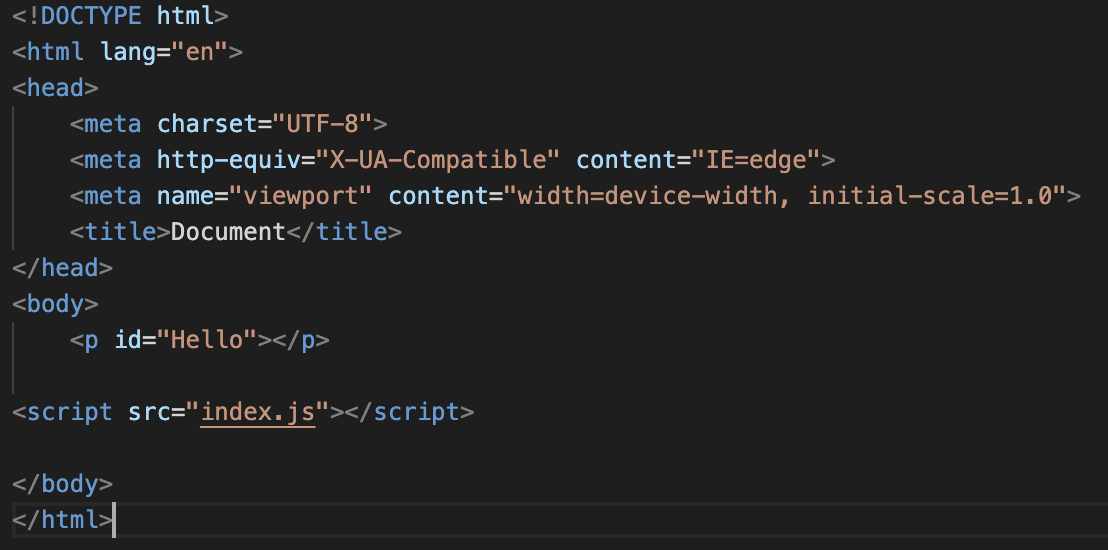
\includegraphics[scale=0.5]{hello}
\end{center}

\subsection{Skrypt walidacyjny}

\begin{center}
	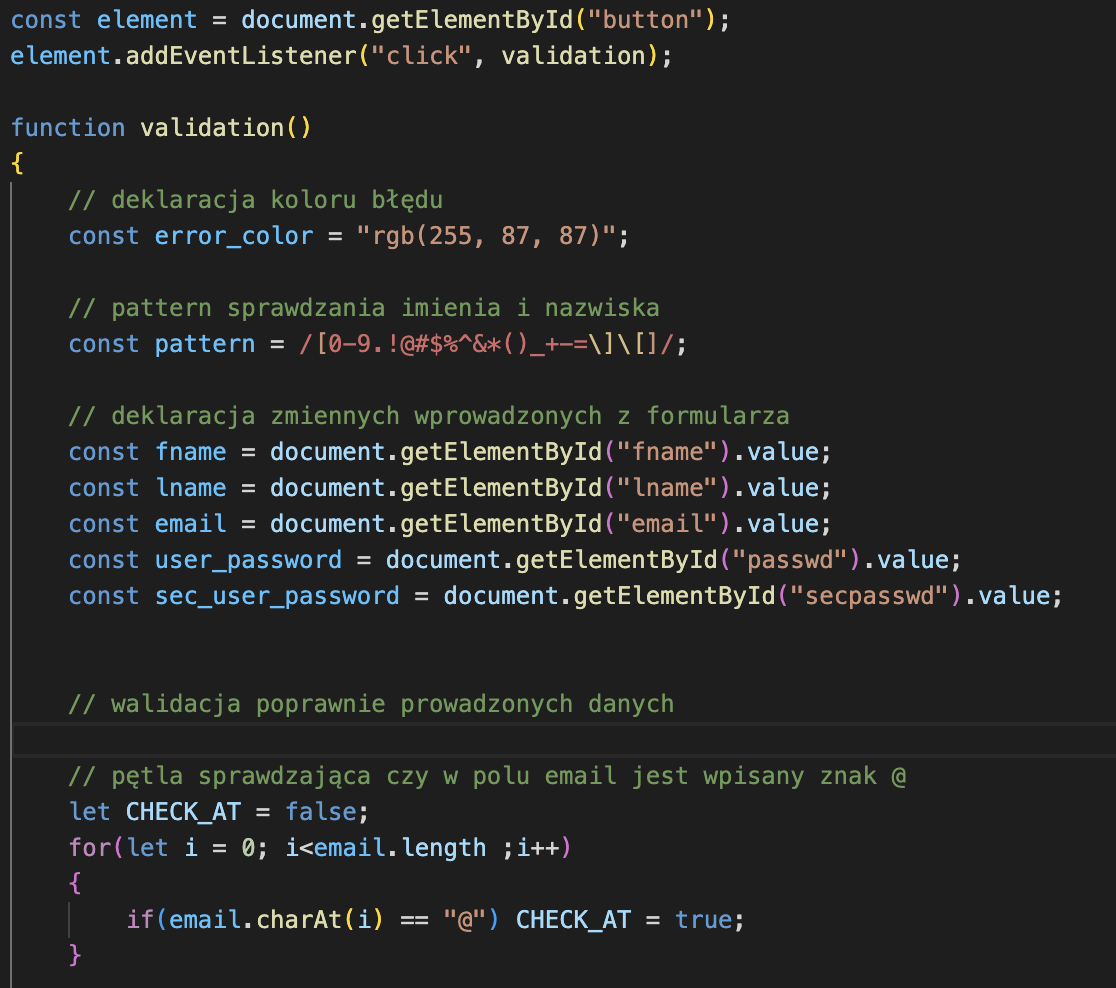
\includegraphics[scale=0.5]{js1}
\end{center}

\begin{center}
	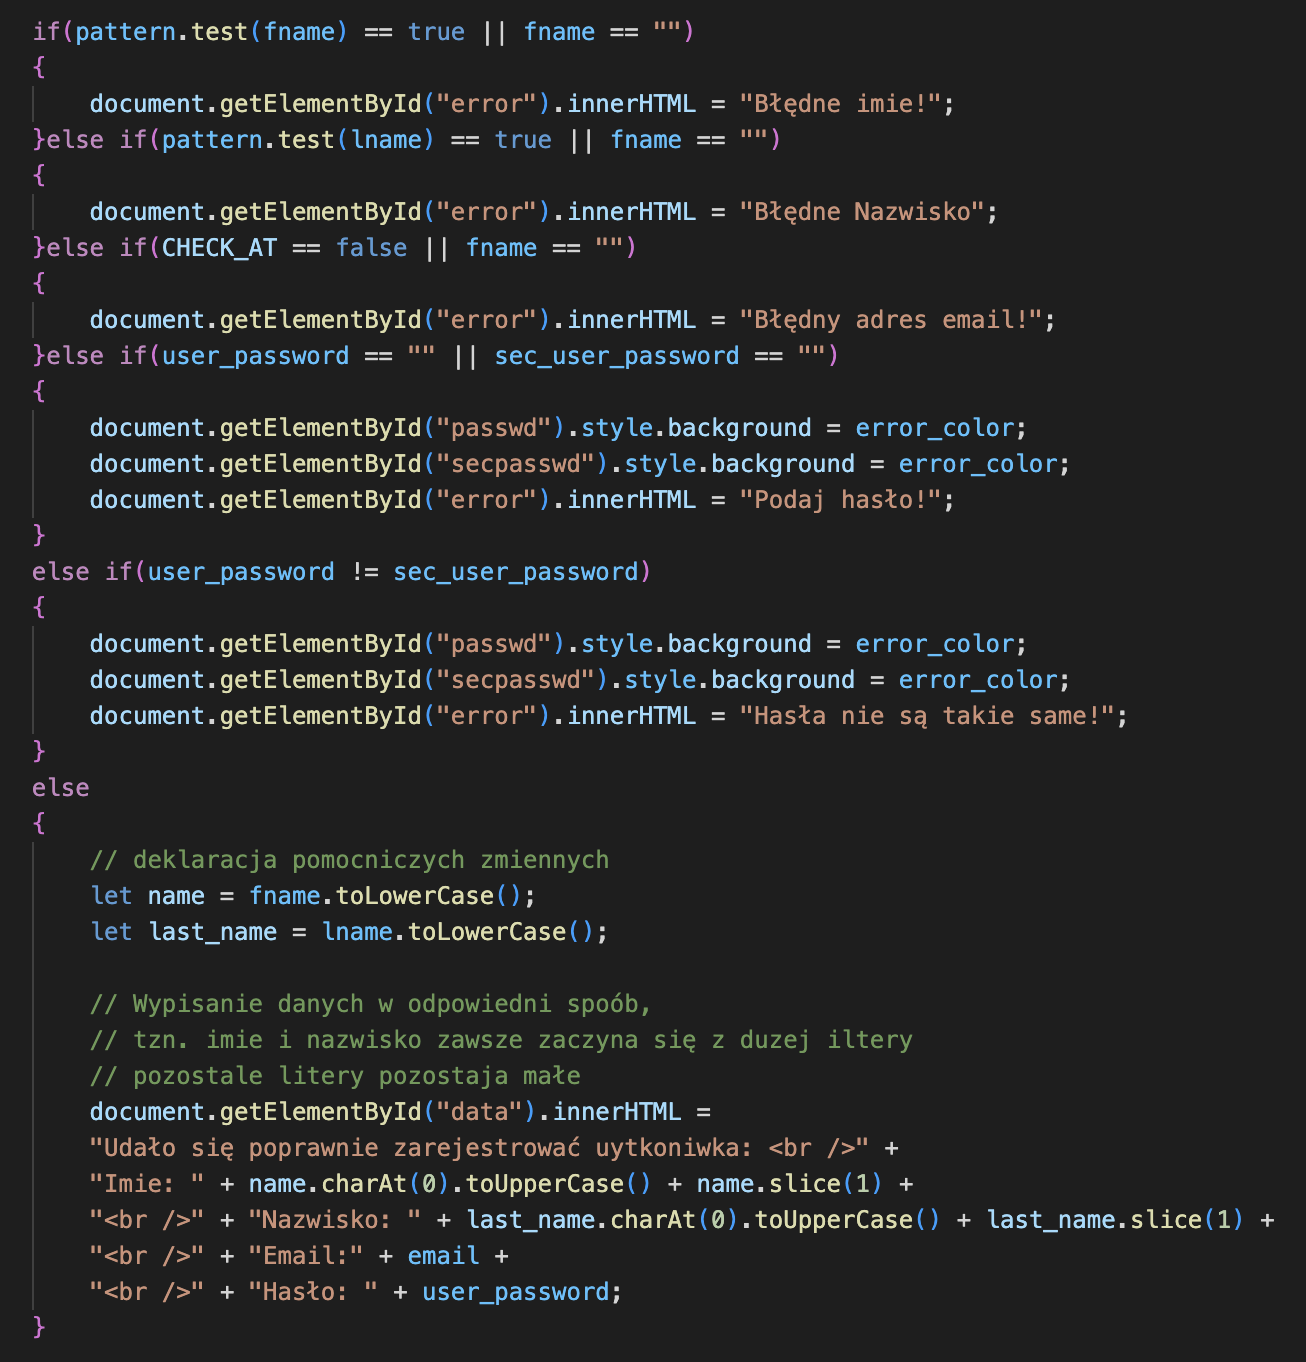
\includegraphics[scale=0.5]{js2}
\end{center}

\section{Opis działania skryptu}

\subsection{Opis zmiennych}
\begin{itemize}
\item error-color => przechowuje dane o kolorze z jakim zostaną wypisane informację błędów,
\item pattern => przechowuje pattern RegExp do sprawdzania imienia i nazwiska,
\item fname => przechowuje imie wpisane przez użytnownika,
\item lname => przechowuje nazwisko wpisane przez użytnownika,
\item email => przechowuje email wpisany przez użytnownika,
\item user-password => przechowuje hasło wpisane przez użytnownika,
\item sec-user-password => przechowuje drugie hasło wpisane przez użytnownika
\end{itemize}

\subsection{Wywołanie skryptu}
\quad Skrypt jest wywołany na końcu pliku index.html w sekcji body, po tym jak użytkownik wpisze dane oraz kliknie przycisk w formularzu. Skrypt jest wywoływany poprzez funkcje addEventListener() podczas kliknięcia.
Funkcja walidacyjna jest umiejscowiona w pliku index.js w funkcji validation().

\section{Opis techniczny projektu}
\begin{itemize}
\item Języki: HTML, JS
\item Środowiska programistyczne: Visual Studio Code
\item Wersja VSC: 1.74.3 (Universal)
\end{itemize}


\end{document}